\chapter{Resultados}

Este capítulo apresenta os resultados obtidos nos experimentos feitos para validação das técnicas utilizadas neste trabalho, bem como o resultado final da aplicação. Buscou-se repetir os experimentos várias vezes (mais do que 30 vezes) a fim de garantir valor estatístico para os resultados apresentados.

\section{Calibração das Câmeras}

A Tabela \ref{tab:params_intrisecos} mostra os parâmetros intrínsecos das câmeras utilizadas, obtidos a partir da ferramenta \textit{Camera Calibration Toolbox for Matlab}.

\begin{table}[!htb]
\centering
\begin{tabular}{|c|c|c|}
\hline
Parâmetros intrínsecos & Câmera 1 (pixel) & Câmera 2 (pixel)\\ \hline
$f_c(1)$ & $854 \pm 4$ &  $834 \pm 6$ \\ \hline
$f_c(2)$ & $858 \pm 4$ & $836 \pm 6$ \\ \hline
$cc(1)$ & $298 \pm 6$ & $300 \pm 7$ \\ \hline
$cc(2)$ & $232 \pm 6$ & $217 \pm 7$ \\ \hline
$alpha_c$ & 0 & 0 \\ \hline
\end{tabular}

\caption{Parâmetros intrínsecos da câmera medidos em pixeis.}
\label{tab:params_intrisecos}
\end{table}

Como pode ser observado os valores de $f_c(1)$ e $f_c(2)$, referentes a distância focal medida em pixeis horizontais e verticais, são bem próximos para ambas as câmeras. Essa verificação valida a aproximação assumida, durante a modelagem, de que câmera possui um pixel quadrado. Portanto, a distância focal utilizada, para efeitos de cálculo, é dada por $f = (f_c(1) + f_c(2))/2$. Os valores são dados em pixeis.

Os resultados similares obtidos para cada uma das câmeras não é ao acaso, visto que as duas câmeras utilizadas são da mesma marca e modelo. Além disso, ambas possuem foco ajustável, o ajuste em cada uma foi feito manualmente e por avaliação visual, de modo a capturar imagens nítidas.

Os parâmetros calculados fornecem os elementos necessários para tornar possível a estimação da profundidade de um ponto alvo, a partir da Equação \ref{eq:3d_Zequation}. Assim, pode-se estimar o valor de $X$ em centímetros, pelas Equações \ref{eq:3d_realX1} e \ref{eq:3d_realX1}, bem como estimar o valor de $Y$ em centímetros, pelas Equações \ref{eq:3d_realY1} e \ref{eq:3d_realY2}.

\section{Rastreamento de Pontos da Face}

Os experimentos realizados nesta seção foram feitos com o objetivo de avaliar isoladamente a precisão da detecção de pontos da face utilizando a SDK \textit{CSIRO Face Analysis}, ou seja, as medidas são tomadas com os valores puros (em pixeis e não filtrados) obtidos pelo rastreamento. O objetivo desta análise é permitir a comparação com os resultados obtidos após filtragem e estimação de tridimensionalidade, bem como justificar o uso destas técnicas.


Escolheu-se medir a razão de distância para o \textbf{comprimento dos lábios} em repetidas tomadas, para duas das poses disponíveis: a Pose Neutra e a Pose Sorrindo. Essa razão de distância, após filtragem, compõe o peso de mistura para a Pose Sorrindo na aplicação final e foi escolhida por ser a razão que apresenta maior amplitude de variação entre os extremos máximos e mínimos.

Para ambas câmeras 1 e 2 obteve-se a média e o desvio padrão, em pixeis, para essa razão de distância. Esses dados foram adquiridos a medida que o usuário se posicionava a diferentes distâncias em relação à montagem de captura, variando, assim, os valores de profundidade. Os dados de média e desvio padrão foram obtidos a partir de medições em trinta imagens de uma face imóvel, capturadas sucessivamente com intervalos de tempo menores que um segundo.

A Tabela \ref{tab:exp-px-variando-dist-cam1} exibe os valores obtidos através da câmera 1 enquanto a Figura \ref{fig:graf-cam1-dsv-dist} mostra um gráfico da variação do desvio padrão do comprimento dos lábios, para a Pose Neutra e a para Sorrindo, em relação a distância entre a câmera 1 e o alvo.


\begin{table}[!htb]
\centering
\begin{tabular}{|*{6}{>{\centering\arraybackslash}p{.16\linewidth}|}}
\cline{2-5}
	\multicolumn{1}{c|}{} & \multicolumn{2}{c|}{Câmera 1 - Pose Neutra (pixel)} & \multicolumn{2}{c|}{Câmera 1 - Pose Sorrindo (pixel)} \\ \hline
    \begin{tabular}{@{}c@{}}Distância da \\ câmera (cm)\end{tabular} & Média &  Desvio padrão & Média &  Desvio padrão \\ \hline
40 & 93.4096 & 0.5575 & 92.1488 & 1.3473 \\ \hline
45 & 83.7242 & 0.6406 & 84.694  & 0.8848 \\ \hline
50 & 75.6548 & 0.7163 & 78.1044 & 1.0881 \\ \hline
55 & 67.9294 & 0.6772 & 69.1071 & 0.9671 \\ \hline
60 & 65.1105 & 0.3884 & 65.8582 & 0.8114 \\ \hline
65 & 58.8054 & 0.3392 & 59.7229 & 0.5219 \\ \hline
70 & 54.7137 & 0.5925 & 55.7597 & 0.6367 \\ \hline
75 & 53.4555 & 0.4781 & 53.7684 & 0.6277 \\ \hline
80 & 49.1185 & 0.3156 & 49.7219 & 0.2373 \\ \hline
\end{tabular}
\caption{Comprimento horizontal dos lábios medido em pixeis a partir de imagens capturadas do rosto alvo pela câmera 1 em distâncias variáveis.}
\label{tab:exp-px-variando-dist-cam1}
\end{table}

\begin{figure}[!htb]
\centering
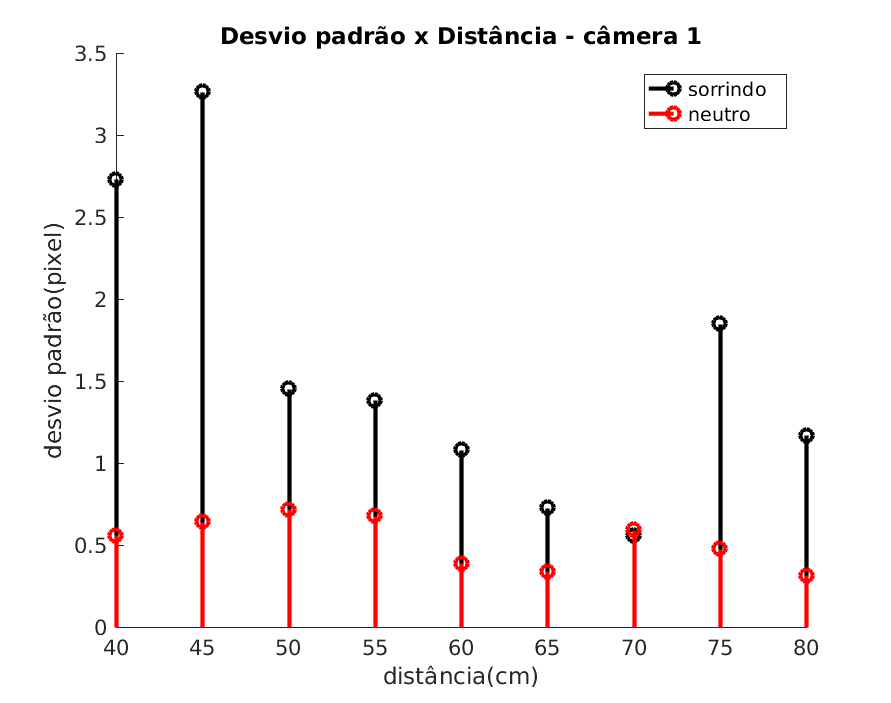
\includegraphics[width=0.8\textwidth]{figs/thumbnail_cameraEsquerda.jpg} 
\caption{Gráfico da variação do desvio padrão, em pixeis, em relação a distância, em centímetros, de pontos rastreados nas imagens capturadas pela câmera 1.}
\label{fig:graf-cam1-dsv-dist}
\end{figure}

A Tabela \ref{tab:exp-px-variando-dist-cam2} exibe os valores obtidos através da câmera 2 e a Figura \ref{fig:graf-cam2-dsv-dist} mostra um gráfico da variação do desvio padrão do comprimento dos lábios, para a Pose Neutra e a para Sorrindo, em relação a distância entre a câmera 2 e o alvo.

\begin{table}[!htb]
\centering
\begin{tabular}{|*{6}{>{\centering\arraybackslash}p{.16\linewidth}|}}
\cline{2-5}
	\multicolumn{1}{c|}{} & \multicolumn{2}{c|}{Câmera 2 - Pose Neutra (pixel)} & \multicolumn{2}{c|}{Câmera 2 - Pose Sorrindo (pixel)} \\ \hline
    \begin{tabular}{@{}c@{}}Distância da \\ câmera (cm)\end{tabular} & Média &  Desvio padrão & Média &  Desvio padrão \\ \hline
40 & 92.1488 & 1.3473 & 119.6076 & 2.2723 \\ \hline
45 & 84.694  & 0.8848 & 106.7452 & 2.23   \\ \hline
50 & 78.1044 & 1.0881 & 108.4763 & 1.2881 \\ \hline
55 & 69.1071 & 0.9671 & 94.7001  & 1.2003 \\ \hline
60 & 65.8582 & 0.8114 & 87.5216  & 0.5491 \\ \hline
65 & 59.7229 & 0.5219 & 82.719   & 0.9558 \\ \hline
70 & 55.7597 & 0.6367 & 75.3994  & 0.4099 \\ \hline
75 & 53.7684 & 0.6277 & 67.9172  & 1.0836 \\ \hline
80 & 49.7219 & 0.2373 & 68.2629  & 1.0946 \\ \hline
\end{tabular}
\caption{Comprimento horizontal dos lábios medido em pixeis a partir de imagens capturadas do rosto alvo pela câmera 2 em distâncias variáveis.}
\label{tab:exp-px-variando-dist-cam2}
\end{table}

\begin{figure}[!htb]
\centering
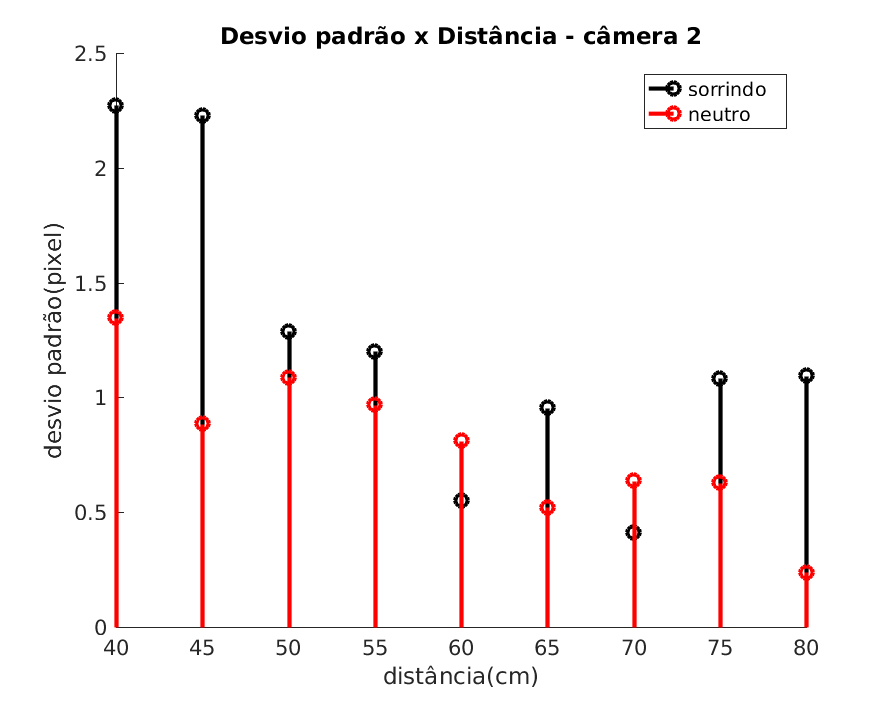
\includegraphics[width=0.8\textwidth]{figs/thumbnail_cameraDireita.jpg} 
\caption{Gráfico da variação do desvio padrão, em pixeis, em relação a distância, em centímetros, de pontos rastreados nas imagens capturadas pela câmera 2.}
\label{fig:graf-cam2-dsv-dist}
\end{figure}

O desvio padrão é importante pois funciona como um indicador da precisão do processo de medida. Fosse o processo regido por uma distribuição puramente Gaussiana, o desvio padrão do processo indicaria que aproximadamente 66\% das medidas serão observadas dentro de uma distância igual ao desvio padrão da média do processo, que é aceito como o valor mais provável para o valor verdadeiro sendo medido.  Os gráficos exibidos na Figura \ref{fig:graf-cam1-dsv-dist} e na Figura \ref{fig:graf-cam2-dsv-dist} mostram que existe incerteza no rastreamento de pontos da face e que a incerteza apresenta um comportamento que varia com a distância. Apesar de o desvio padrão ter sido pequeno quando comparado às dimensões de cada uma das das imagens capturadas, a existência dessa imprecisão pode afetar a qualidade da aplicação final. Além disso, outra análise interessante é que, como as imagens onde o rastreamento foi aplicado foram tomadas em intervalos de tempo muito curtos, e, ainda assim, houve variação nas medidas realizadas, diz-se que essas variações constituem um sinal de erro que deve possuir componentes de elevada frequência. Isto é, o ruído presente no processo de medida deve possuir componentes rápidas o suficiente para que seja capaz de influenciar medidas tomadas em instantes de tempo muito próximos uns dos outros. Essa observação motiva o uso de filtragem digital com o objetivo de cortar tais altas frequências.

Outro comportamento exibido pelos gráficos é o de que o desvio padrão é quase sempre maior quando a razão de distância é medida na Pose Sorrindo, do que quando ela é medida na Pose Neutra, ou seja, o rastreamento geralmente é mais preciso quando tomado em uma face sem expressões.  Este resultado pode ser um reflexo do erro de truncamento introduzido pela escolha de apenas algumas das configurações encontradas pela análise PCA e que, aparentemente, as componentes escolhidas privilegiam configurações neutras.

Outra observação que pode ser tirada é que o desvio padrão em geral diminui com o aumento da distância. Esse acontecimento pode ser atribuído ao fato de que, como neste experimento as medidas são avaliadas em pixeis, quanto maior a distância do usuário a câmera menor o valor da razão de distância.

Finalmente, observando as tabelas é possível reparar a diminuição drástica da média das medidas conforme o valor de profundidade aumenta: vê-se que o valor obtido para o comprimento dos lábios a uma distância de 80cm é quase a metade do valor obtido a 40cm.  Essa mudança brusca impossibilita uma boa determinação das distâncias mínimas e máximas, necessárias para a boa calibração de uma razão de distância, uma vez que estes parâmetros mudam com uma variação de profundidade, mesmo se o alvo estiver na mesma pose.

Estas duas últimas observações motivam o uso de uma técnica de medida que produza valores invariantes a distância que o usuário se encontra do sistema de captura. Esta técnica deve produzir sempre uma mesma razão de distância para uma mesma pose, independentemente da proximidade do usuário nas imagens de entrada.

\section{Estimação de Tridimensionalidade	}

O objetivo dos experimentos nessa seção é avaliar a precisão da técnica de estimação tridimensional. Deve-se notar que uma precisão na estimação do $X$ e do $Y$ no sistema de coordenadas do mundo só é possível caso haja precisão na estimação do $Z$, como pode ser observado nas Equações \ref{eq:3d_realX1}, \ref{eq:3d_realX2}, \ref{eq:3d_realY1} e \ref{eq:3d_realY2}.

Como nos experimentos da seção anterior, a razão de distância analisada foi a referente ao comprimento dos lábios. Foram utilizadas as mesmas imagens capturadas no experimento anterior, porém desta vez as medidas foram tomadas após o par de imagens ter sido combinado com os parâmetros intrínsecos da câmera para produzir medidas em centímetros, ou seja, os pontos foram estimados no sistema de coordenadas do mundo.

A Tabela \ref{tab:exp-px-variando-dist-3d} exibe os valores estimados em centímetros para a média e o desvio padrão do comprimento dos lábios para as poses Neutra e Sorrindo. Já a Figura \ref{fig:graf-3d-dsv-dist} e a Figura \ref{fig:graf-3d-media-dist} mostram gráficos para estes valores a medida que o usuário se afasta do sistema de captura.


\begin{table}[!htb]
\centering
\begin{tabular}{|*{6}{>{\centering\arraybackslash}p{.16\linewidth}|}}
\cline{2-5}
	\multicolumn{1}{c|}{} & \multicolumn{2}{c|}{Pose Neutra (cm)} & \multicolumn{2}{c|}{ Pose Sorrindo (cm)} \\ \hline
    \begin{tabular}{@{}c@{}}Distância da \\ câmera (cm)\end{tabular} & Média &  Desvio padrão & Média &  Desvio padrão \\ \hline
40 & 5.2755 & 0.1155 & 6.8652 & 0.2549 \\ \hline
45 & 5.5857 & 0.0991 & 6.8311 & 0.1564 \\ \hline
50 & 5.4356 & 0.0959 & 7.3474 & 0.116  \\ \hline
55 & 5.3663 & 0.1135 & 7.3599 & 0.1574 \\ \hline
60 & 5.5722 & 0.1144 & 7.4396 & 0.1107 \\ \hline
65 & 5.4381 & 0.0932 & 7.4996 & 0.1433 \\ \hline
70 & 5.8243 & 0.0879 & 7.7648 & 0.1024 \\ \hline
75 & 5.7759 & 0.1494 & 7.1711 & 0.2339 \\ \hline
80 & 5.5645 & 0.0716 & 7.7803 & 0.1659 \\ \hline
\end{tabular}
\caption{Comprimento horizontal dos lábios medido em centímetros a partir de imagens capturadas do rosto alvo em distâncias variáveis.}
\label{tab:exp-px-variando-dist-3d}
\end{table}

\begin{figure}[!htpb]
\centering
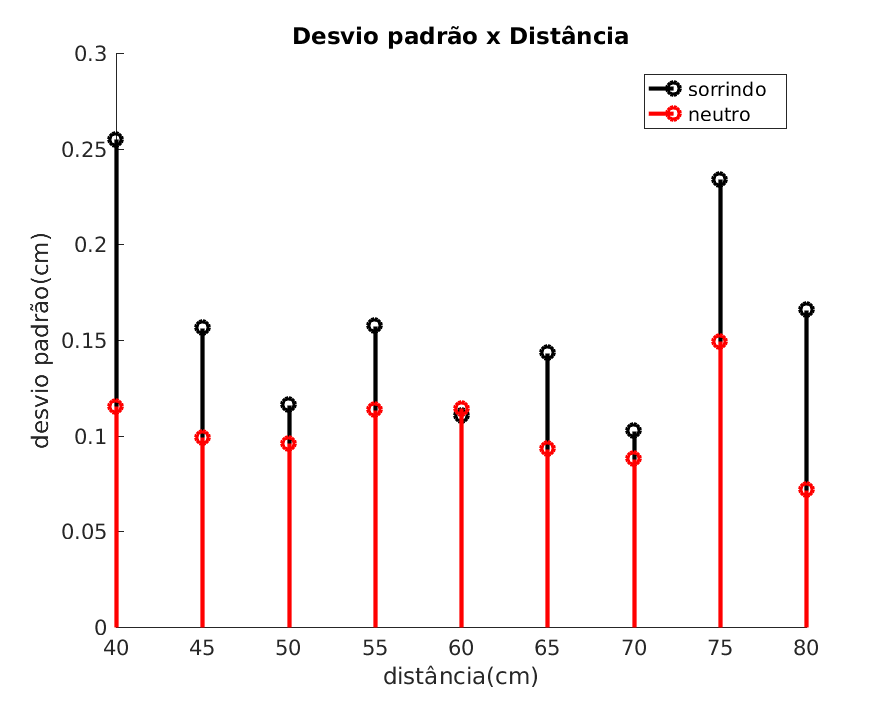
\includegraphics[width=0.8\textwidth]{figs/thumbnail_distanciaCorrigida.jpg} 
\caption{Gráfico da variação do desvio padrão, em centímetros, em relação a distância, em centímetros, de pontos estimados no sistema de coordenadas do mundo.}
\label{fig:graf-3d-dsv-dist}
\end{figure}

O gráfico exibido na Figura \ref{fig:graf-3d-dsv-dist} mostra como se comporta o desvio padrão a medida que o usuário se distancia do sistema de captura. O comportamento é similar ao observado nas Figuras \ref{fig:graf-cam1-dsv-dist} e \ref{fig:graf-cam2-dsv-dist}, revelando a característica estocástica do processo de medida adotado. A diferença entre as Figuras  \ref{fig:graf-3d-dsv-dist}, \ref{fig:graf-cam1-dsv-dist} e \ref{fig:graf-cam2-dsv-dist} é que a primeira apresenta os resultado quando as medidas são tomadas no sistema de coordenadas estimadas do mundo enquanto as últimas apresentam resultados quando medidas são tomadas diretamente nos planos das câmeras. Vê-se que a estimação de profundidade não altera este comportamento do sistema de medida.

\begin{figure}[!htpb]
\centering
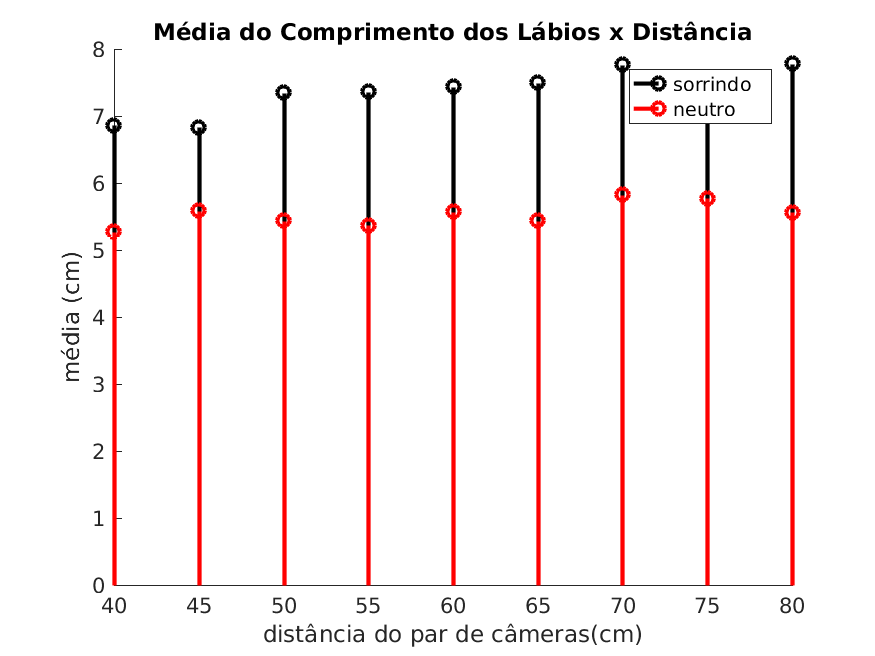
\includegraphics[width=0.8\textwidth]{figs/media3d.png} 
\caption{Gráfico da variação média, em centímetros, em relação a distância, em centímetros, de pontos estimados no sistema de coordenadas do mundo.}
\label{fig:graf-3d-media-dist}
\end{figure}

A precisão da estimação tridimensional pode ser verificada ao se avaliar a variação da média em relação a distância. Esses dados são exibidos na Figura \ref{fig:graf-3d-media-dist}, nota-se que a média se mantém aproximadamente constante, principalmente nos intervalos entre 50cm e 65cm. Com isso pode-se concluir que mesmo que aconteça uma variação da distância do alvo em relação as câmeras, a razão de distância se manterá estável, garantindo estabilidade para o modelo final.

\section{Filtros}

Nestes experimentos foram gerados gráficos para as sequências dos pesos de mistura com e sem filtragem de três das poses utilizadas. Cada gráfico mostra medidas de pesos de mistura para uma das poses, com um curva para os valor não-filtrado e curvas para saídas de alguns dos filtros projetados.  As sequências foram obtidas em um vídeo gravado com o objetivo de movimentar especificamente a pose sendo testada. Os gráficos foram gerados selecionando-se manualmente parte das sequências gravadas que produziram comportamento interessante para comparação.

A Figuras \ref{fig:filter-left-eye}, \ref{fig:filter-open-mouth} e \ref{fig:filter-smile} mostram a atuação dos filtros sobre a variação do peso de mistura para as poses Olho Esquerdo, Boca Aberta e Sorriso respectivamente. Nestes gráficos, mostra-se sempre a saída não filtrada, a saída filtrada com filtro de média móvel de Hanning e a saída filtrada com filtro de projeto com janela de Hamming para algumas frequências de corte. Os filtros com projeto em janela tem todos comprimento 16.

\begin{figure}[!htb]
\centering
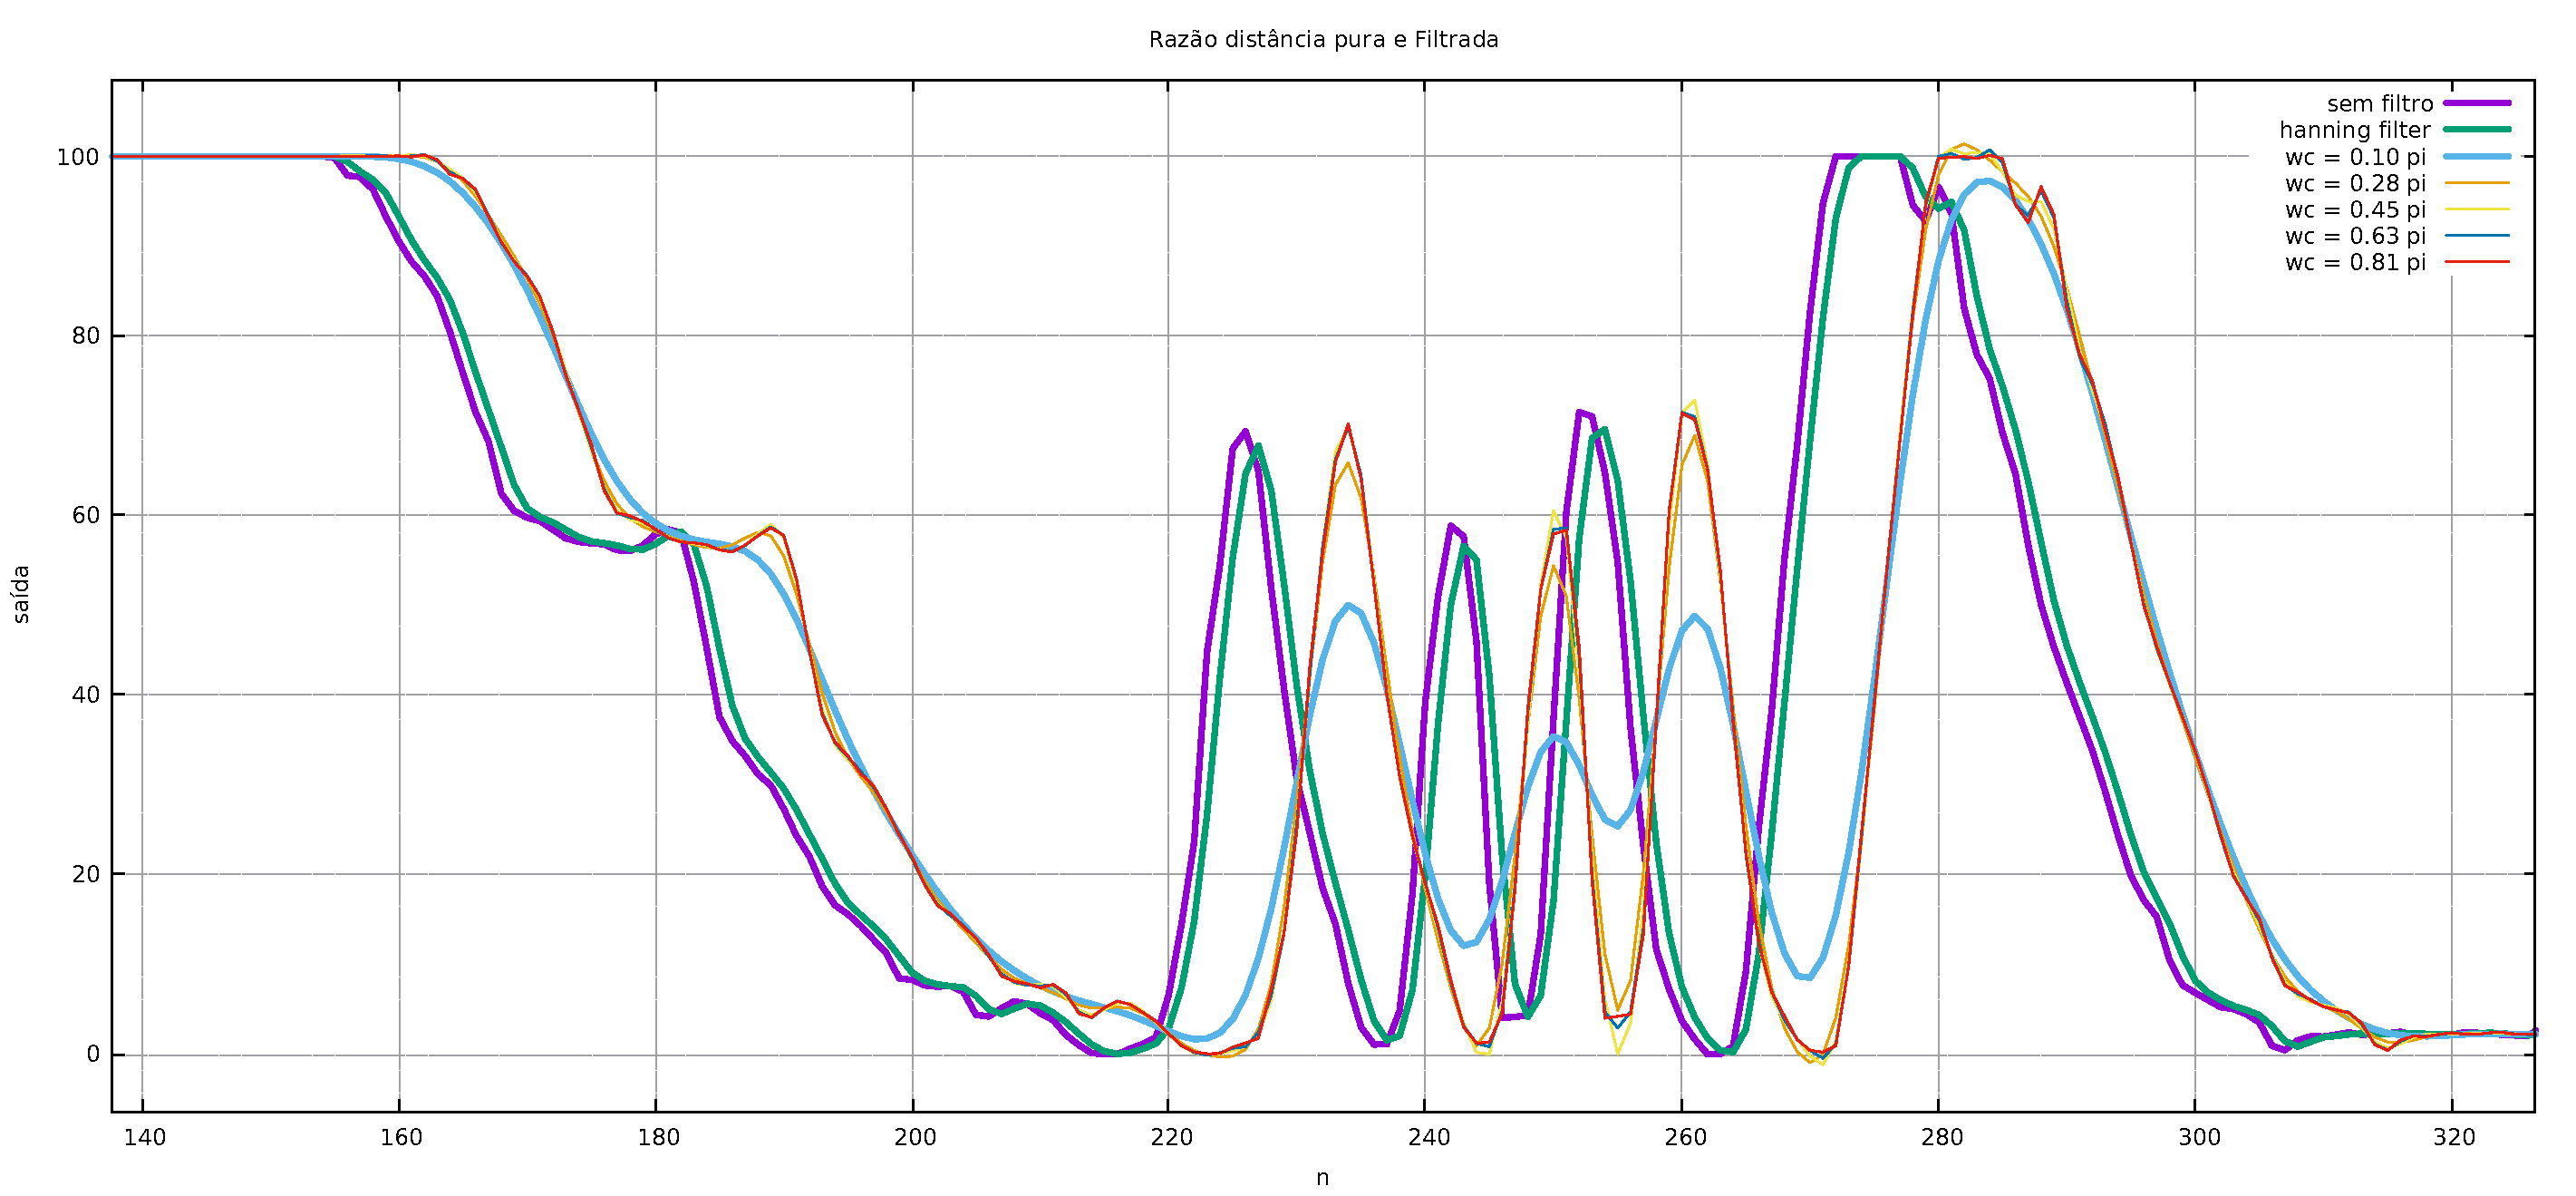
\includegraphics[width=1.0\textwidth]{figs/filter-result-open-mouth.pdf} 
\caption{Peso de mistura para a Pose Olho Esquerdo}
\label{fig:filter-left-eye}
\end{figure}

\begin{figure}[!htb]
\centering
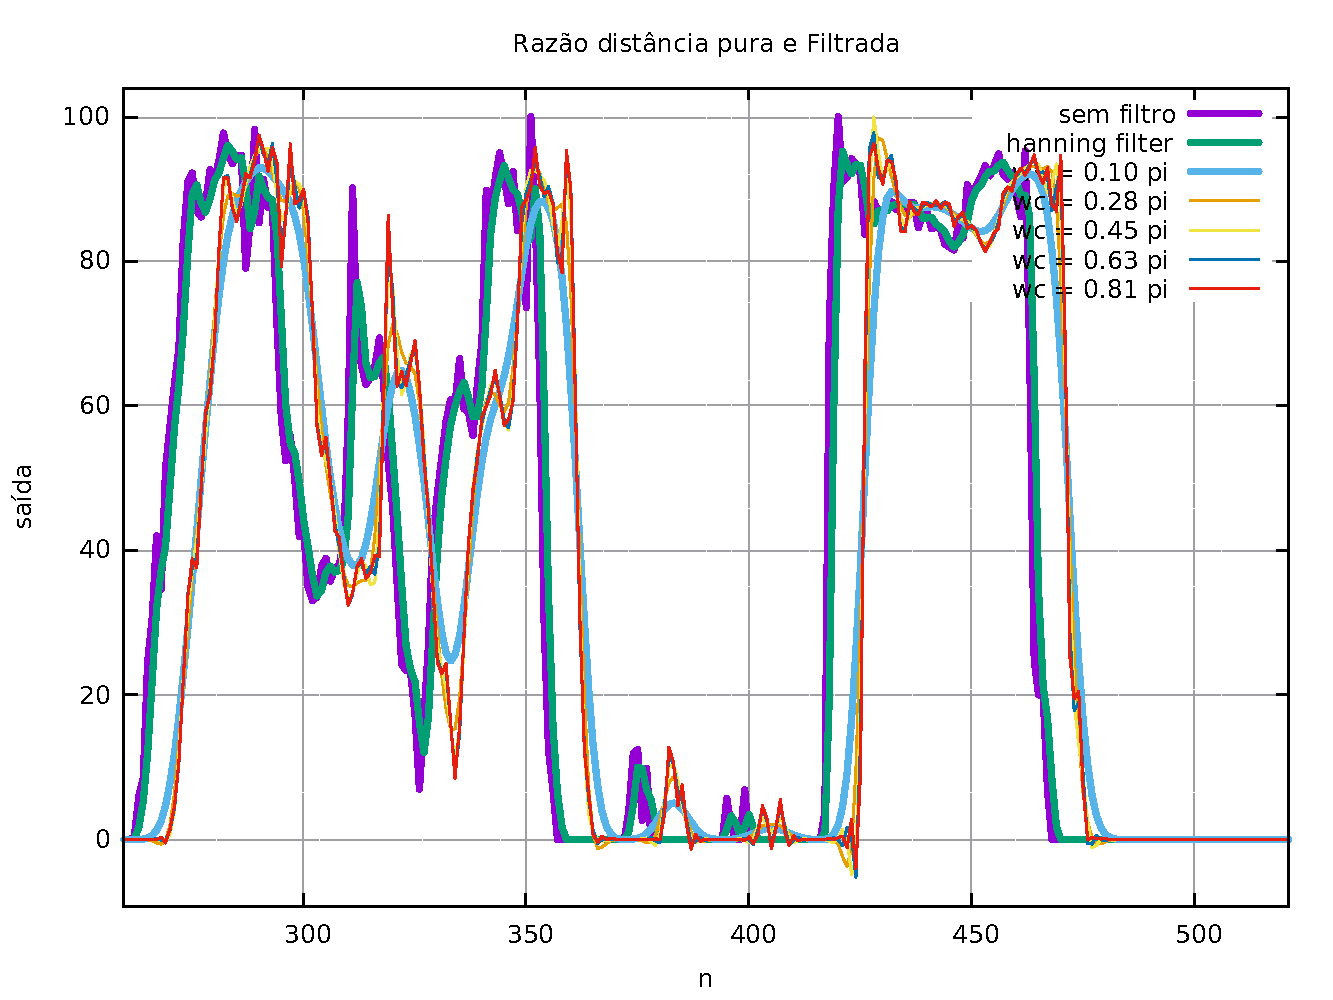
\includegraphics[width=1.0\textwidth]{figs/filter-result-left-eye.pdf} 
\caption{Peso de mistura para a Pose Boca Aberta}
\label{fig:filter-open-mouth}
\end{figure}

\begin{figure}[!htb]
\centering
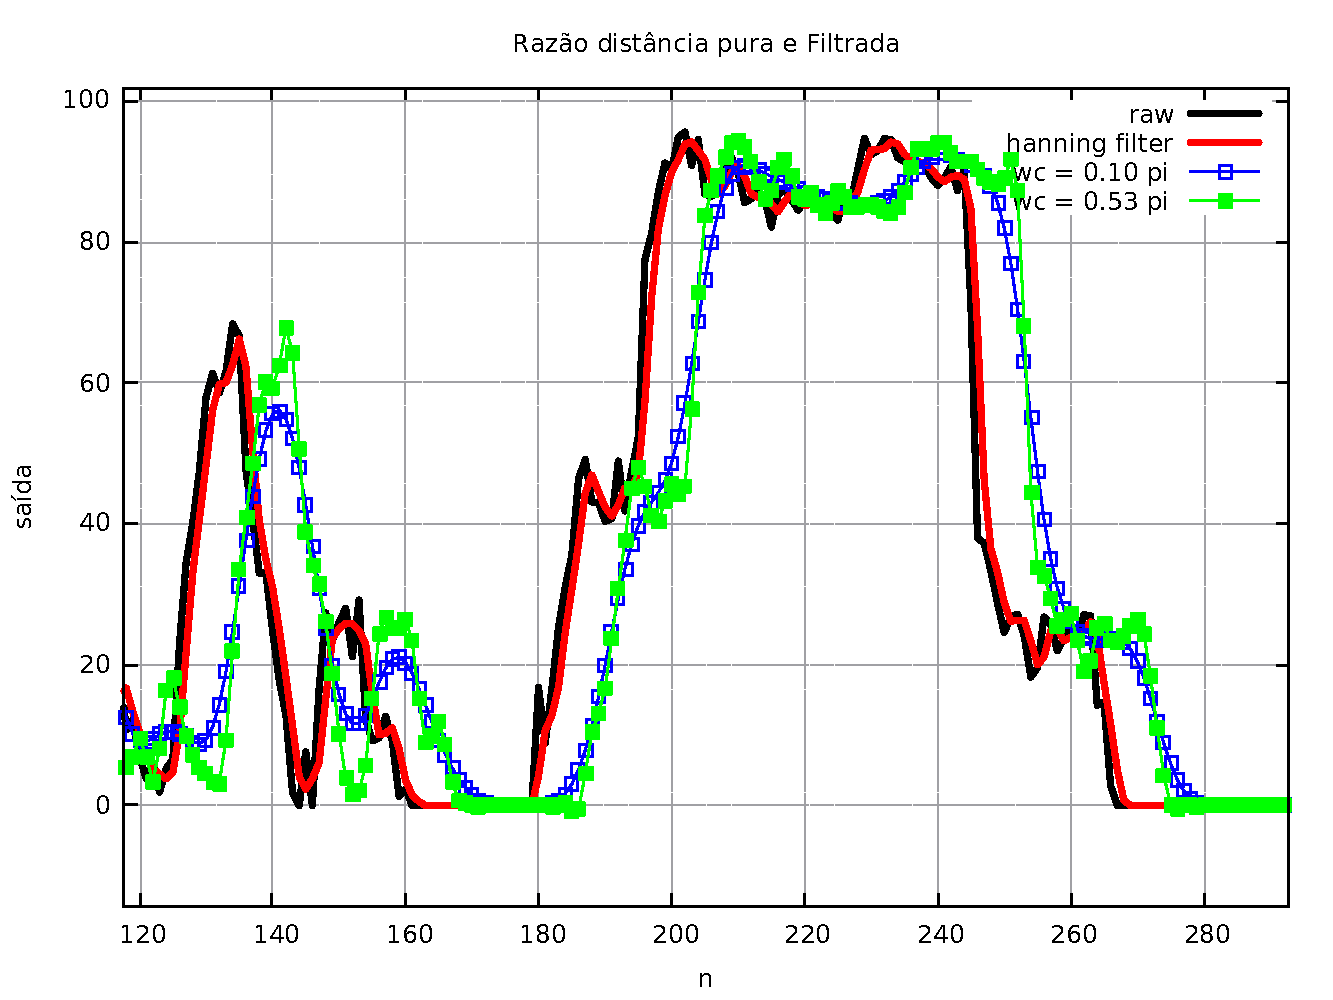
\includegraphics[width=1.0\textwidth]{figs/filter-result-smile.pdf} 
\caption{Peso de mistura para a Pose Sorriso}
\label{fig:filter-smile}
\end{figure}

Como visto nas Figuras \ref{fig:graf-cam1-dsv-dist} e \ref{fig:graf-cam2-dsv-dist} dos experimentos anteriores, o rastreamento em si apresenta instabilidades mesmo quando o rosto está imóvel. Portanto, pode-se esperar que em um vídeo longo onde ocorre movimentação e variação de luminosidade o sinal sem filtragem seja ainda mais instável. Esse comportamento é visto nas oscilações rápidas observadas nos gráficos em \ref{fig:filter-left-eye}, \ref{fig:filter-open-mouth} e \ref{fig:filter-smile}. 

A filtragem suaviza o sinal e consequentemente remove oscilações indesejáveis na animação final. Vários tipos de filtro foram analisados e seus desempenhos foram variados. Como pode ser observado, os filtros projetados pela técnica de janela foram compridos de mais e introduzem atrasos no sinal de saída em relação ao de entrada sinal e, apesar de eles serem mais poderosos em filtrar altas frequências, esse tipo de filtro acaba prejudicando a performance da animação em tempo real. 

Por outro lado o filtro de média móvel de Hanning segue adequadamente o sinal original e mantem uma boa atenuação das altas frequências. Esse filtro introduz um menor atraso em seguir o sinal de entrada, pois possui muito menos coeficientes que os outros filtros projetados. Para este trabalho, onde um dos objetivos é a animação em tempo real, o filtro de Hanning apresentou o melhor resultado. Poderia ter sido experimentado um projeto em janela utilizando-se menos coeficientes, mas como o filtro de média móvel mostrou bons resultados, decidiu-se por não prosseguir com a experimentação de mais filtros.

\section{Mistura de Poses}

Neste experimento trabalhou-se apenas com a técnica de Mistura de Poses para compor um modelo final sem a influência do rastreamento de pontos da face. Isto foi feito para ser possível avaliar esta técnica isoladamente. Para isso foram atribuídos manualmente os valores dos pesos de mistura.

Alguns exemplos de modelos finais mostrando poses intermediárias renderizadas com sucesso podem ser vistos na Figura \ref{fig:blend-shapes-inter-simple-shapes}.

\begin{figure}[!htb]
  \centering
  \begin{subfigure}[]{\label{fig:inter1}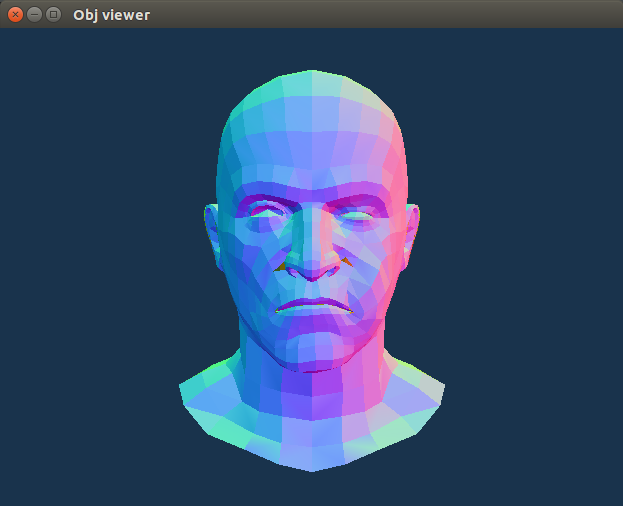
\includegraphics[width=0.4\textwidth]{./figs/TG_angry60_leftcheek75_lefteye55_closemouth35.png}}
  \end{subfigure}   
  \begin{subfigure}[]{\label{fig:inter2}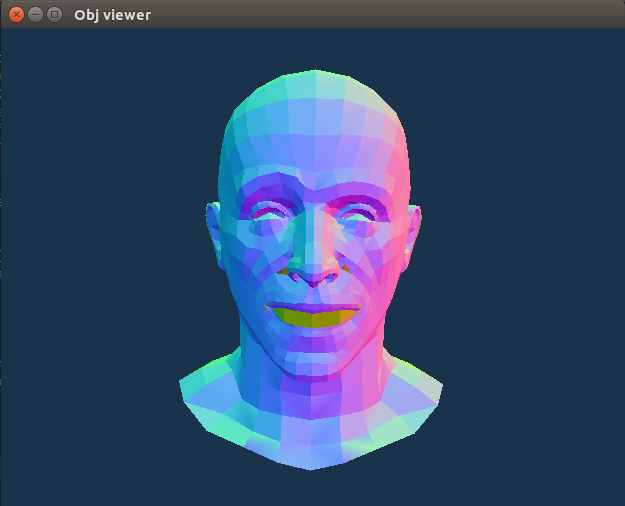
\includegraphics[width=0.4\textwidth]{./figs/TG_happy40_righteyebrow95_openmouth60.png}}
  \end{subfigure}
  
  \begin{subfigure}[]
  {\label{fig:inter3}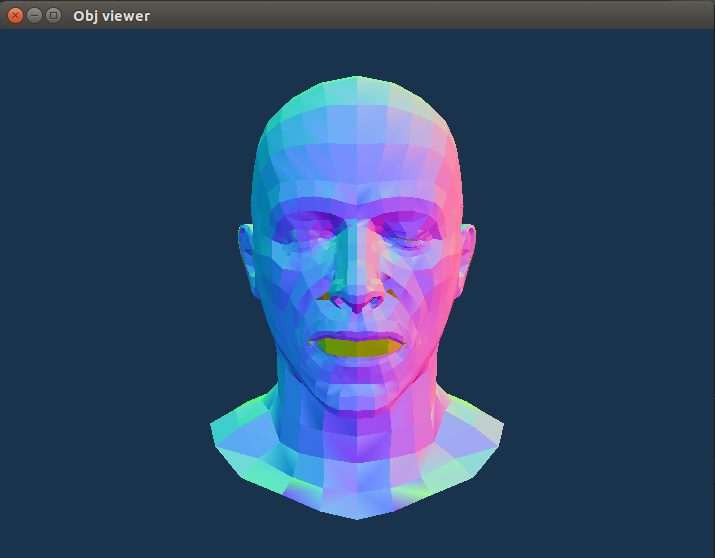
\includegraphics[width=0.4\textwidth]{./figs/TG_lefteye100_rigtheye100_openmouth60.png}}
  \end{subfigure} 
  \begin{subfigure}[]
  {\label{fig:inter4}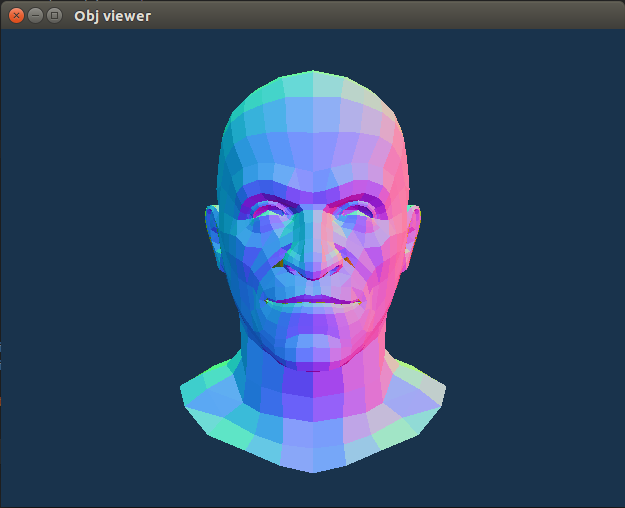
\includegraphics[width=0.4\textwidth]{./figs/TG_happy70_angry90.png}}
  \end{subfigure}
  
  \begin{subfigure}[]{\label{fig:inter5}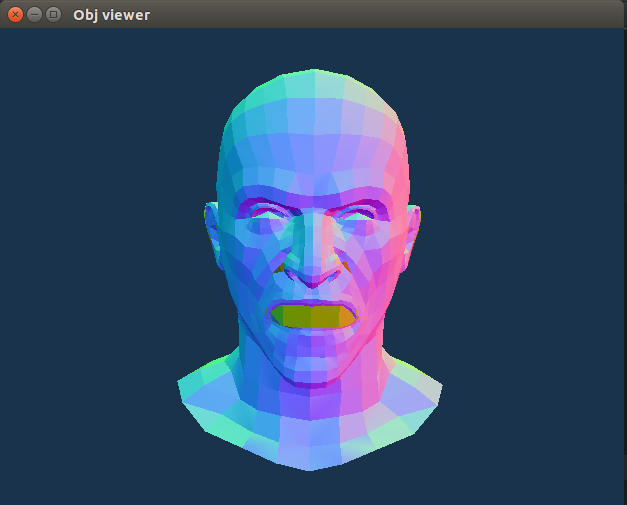
\includegraphics[width=0.4\textwidth]{./figs/TG_angry100_openmouth90.png}}
  \end{subfigure}
  \begin{subfigure}[]{\label{fig:inter6}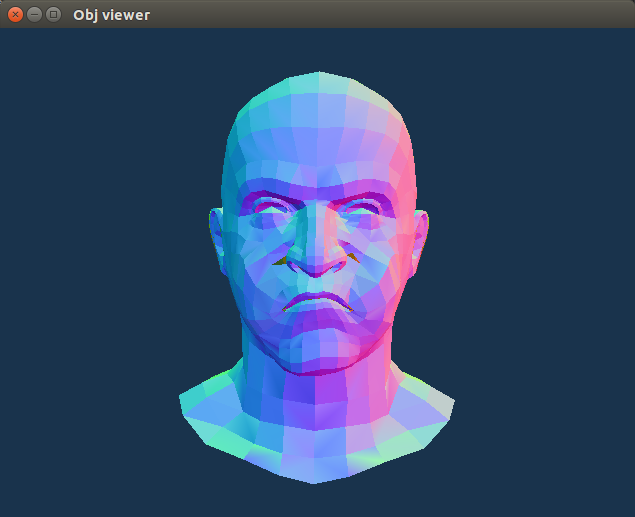
\includegraphics[width=0.4\textwidth]{./figs/TG_angry100_leftcheek100_rightcheek65_closemouth100.png}}
  \end{subfigure}

  \caption{Exemplo de misturas geradas configurando os parâmetros de mistura manualmente. Pesos da Figura \ref{fig:inter1}: Olho Esquerdo - 0.55, Boca Fechada - 0.35, Bochecha Esquerda - 0.75 e Bravo - 0.6. Pesos da Figura \ref{fig:inter2}: Sobrancelha Direita - 0.95, Boca Aberta - 0.6 e Sorrindo - 0.4. Pesos da Figura \ref{fig:inter3}: Olho Esquerdo - 1.0, Olho Direito - 1.0 e Boca Aberta - 0.6. Pesos da Figura \ref{fig:inter4}: Sorrindo - 0.7 e Bravo - 0.6. Pesos da Figura \ref{fig:inter5}: Boca Aberta - 1.0 e Bravo - 0.9. Pesos da Figura \ref{fig:inter6}: Boca Fechada - 1.0, Bochecha Esquerda - 1.0, Bochecha Direita - 0.65, e Bravo - 1.0.}

  \label{fig:blend-shapes-inter-simple-shapes}
\end{figure}

Como pode ser observado nos modelos exibidos, a técnica de mistura de poses teve ótimos resultados. Os resultados mostram que a implementação utilizando  indexação de VBOs e que a ordenação dos vetores foi adequada. Não fosse esse o caso, seria possível observar falhas no modelo, como  buracos ou presença de deformações irregulares.

Pode-se notar que a presença de cada pose chave no modelo final está bem relacionada com os pesos aplicados. Verifica-se que a aplicação da Equação \ref{eq:blendshapes} permite criar, a partir de poucas poses pré-definidas, uma quantidade enorme de poses intermediárias significativamente diferentes.

Com esses resultados nota-se que se o programa for capaz 
de gerar pesos de mistura que adequadamente correspondam às expressões apresentadas pelo usuário, a técnica de mistura de poses será capaz de compor um modelo final com expressões variadas.

\section{Sistema em Funcionamento}

Para que o sistema funcione adequadamente é necessária uma etapa de calibração das distâncias mínimas e máximas observadas em cada uma das razões de distância. Isso é feito de forma manual ao executar o programa, pois toma-se nota de valores impressos em tela sobre as distâncias entre os pontos tomadas no quadro atual. Por exemplo, pode-se sorrir e, então, anotar o valor medido para o sorriso que é impresso na tela. Os valores anotados são, posteriormente, inseridos no código para serem utilizados para cálculo das razões de distância. Os valores utilizados para a sequência de resultados obtidos a seguir são apresentados na Tabela \ref{tab:distance-ratio-coeffs}.

\begin{table}
\centering
\begin{tabular}{|c|c|c|}
\hline
pose & distância mínima (cm) & distância mínima (cm) \\ \hline
sorriso & 5.9 & 7.9 \\ \hline
sobrancelha esquerda & 2.4 & 3.7 \\ \hline
sobrancelha direita & 2.4 & 3.6 \\ \hline
olho esquerdo & 0.3 & 0.6 \\ \hline
olho direito & 0.3 & 0.6 \\ \hline
boca aberta & 0.3 & 4.3 \\ \hline
\end{tabular}
\caption{Valores de distância mínima e distância máxima definidos, para cada pose, após calibração.}
\label{tab:distance-ratio-coeffs}
\end{table}

Utiliza-se os coeficientes acima para rodar a aplicação sobre vídeos de entrada e guarda-se alguns quadros dos vídeos e da saída.
As Figuras \ref{fig:sist-func}, \ref{fig:sist-func-2}, \ref{fig:sist-func-3} e \ref{fig:sist-func-4} mostram lado a lado quadros de entrada e os resultados da transferência de expressão para o avatar. Nas Figuras de \ref{fig:sist-func} a \ref{fig:sist-func-3} os quadros de entrada foram escolhidos de forma a mostrar expressões variadas que podem ser capturadas pela técnica proposta. A figura \ref{fig:sist-func-4} mostra uma sequência de três quadros consecutivos tirada enquanto o usuário conversava com a câmera. Notar que a boca do avatar abre seguindo o movimento do usuário.

Os resultados mostram que o acoplamento entre o rastreamento de pontos do rosto com os pesos de mistura por meio de razões de distâncias se deu de forma satisfatória. Há poses para mistura que não foram utilizadas, mas todas as poses para as quais se definiu uma razão de distância foram adequadamente transferidas do usuário para o avatar. O avatar é capaz de sorrir, abrir a boca, movimentar as sobrancelhas e piscar segundo o movimento do usuário. 


\begin{figure}[!htb]
  \centering
  \begin{subfigure}[]{\label{fig:inter1}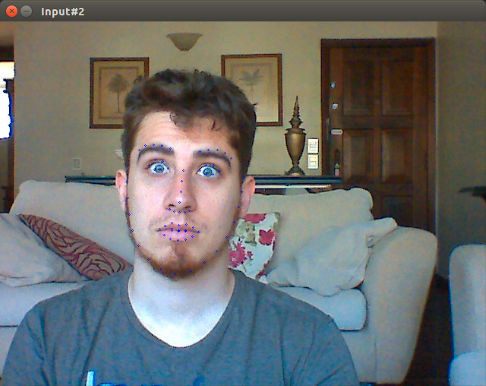
\includegraphics[width=0.35\textwidth]{./figs/TG-resultado-par-4-img-1.png}}
  \end{subfigure}   
  \begin{subfigure}[]{\label{fig:inter2}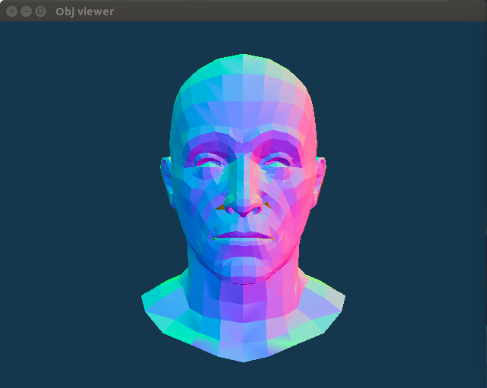
\includegraphics[width=0.35\textwidth]{./figs/TG-resultado-par-4-img-2.png}}
  \end{subfigure}
  
  \begin{subfigure}[]
  {\label{fig:inter3}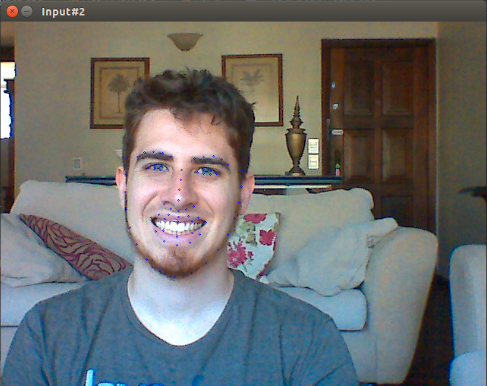
\includegraphics[width=0.35\textwidth]{./figs/TG-resultado-par-5-img-1.png}}
  \end{subfigure} 
  \begin{subfigure}[]
  {\label{fig:inter4}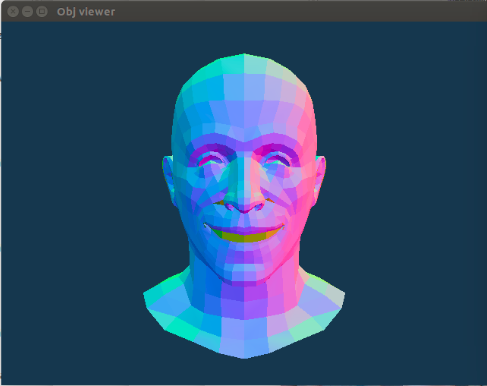
\includegraphics[width=0.35\textwidth]{./figs/TG-resultado-par-5-img-2.png}}
  \end{subfigure}
  
    \begin{subfigure}[]
  {\label{fig:inter3}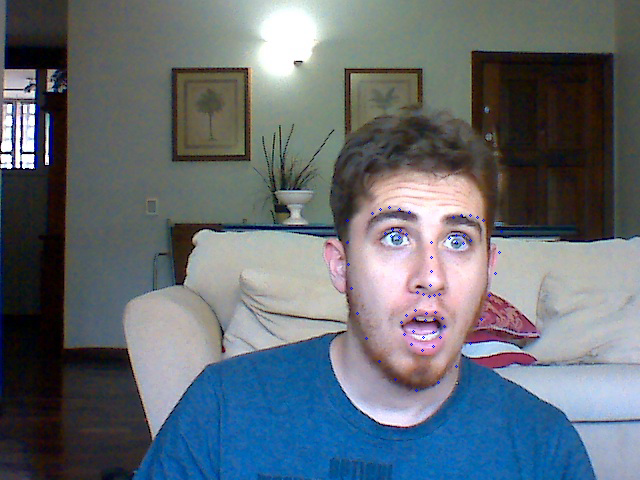
\includegraphics[width=0.35\textwidth]{./figs/i_0230.png}}
  \end{subfigure} 
  \begin{subfigure}[]
  {\label{fig:inter4}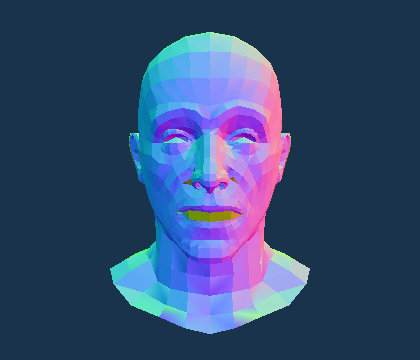
\includegraphics[width=0.35\textwidth]{./figs/o_0250.png}}
  \end{subfigure}

  \caption{Imagens que demonstram o sistema em funcionamento.  Em relação ao movimento da boca, as Figuras \ref{fig:sist-func}(d) e \ref{fig:sist-func}(f) deixam claro que há dois movimentos sendo rastreados independentemente: abrir a boca verticalmente como no ato de bocejar e abri-la horizontalmente como no ato de sorrir.}

  \label{fig:sist-func}
\end{figure}

\begin{figure}[!htb]
  \centering
  \begin{subfigure}[]{\label{fig:inter1}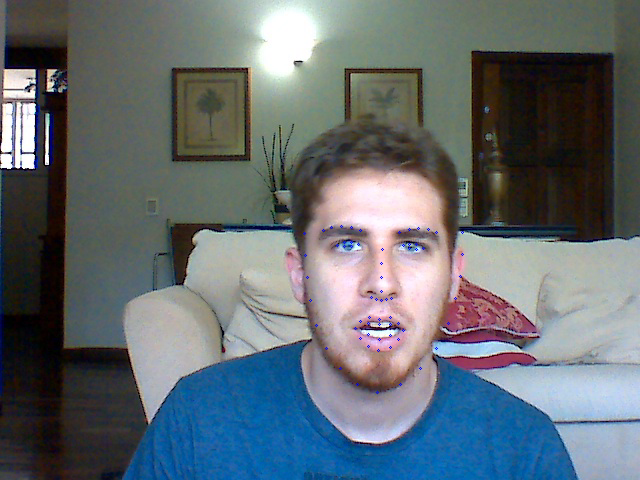
\includegraphics[width=0.35\textwidth]{./figs/i_0330.png}}
  \end{subfigure}   
  \begin{subfigure}[]{\label{fig:inter2}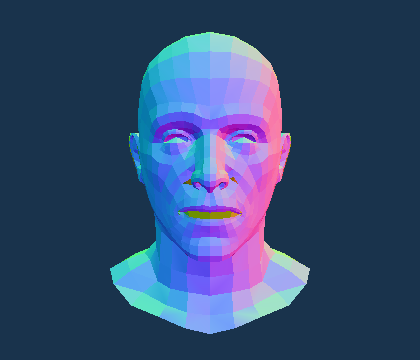
\includegraphics[width=0.35\textwidth]{./figs/o_0370.png}}
  \end{subfigure}
  
  \begin{subfigure}[]
  {\label{fig:inter3}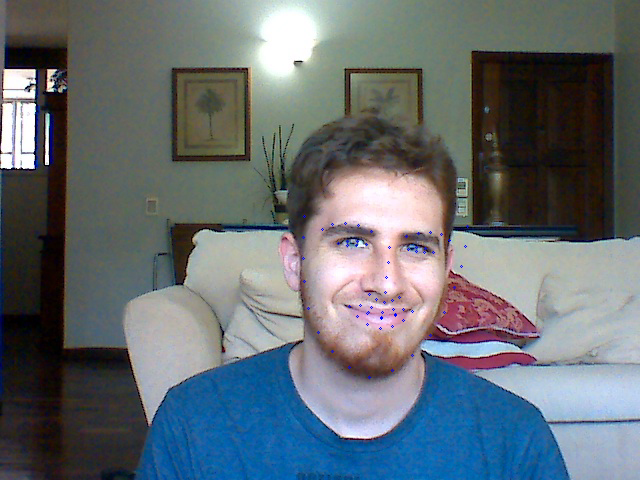
\includegraphics[width=0.35\textwidth]{./figs/i_0350.png}}
  \end{subfigure} 
  \begin{subfigure}[]
  {\label{fig:inter4}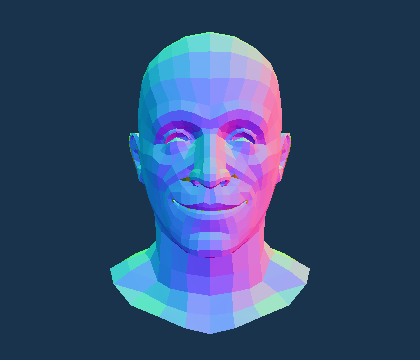
\includegraphics[width=0.35\textwidth]{./figs/o_0380.png}}
  \end{subfigure}
  
    \begin{subfigure}[]
  {\label{fig:inter3}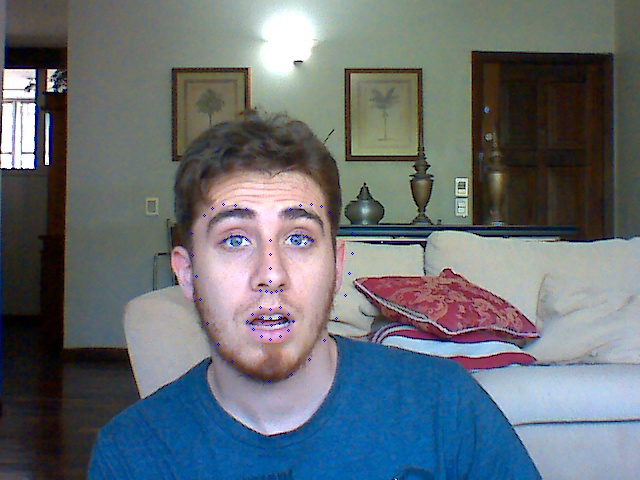
\includegraphics[width=0.35\textwidth]{./figs/i_0550.png}}
  \end{subfigure} 
  \begin{subfigure}[]
  {\label{fig:inter4}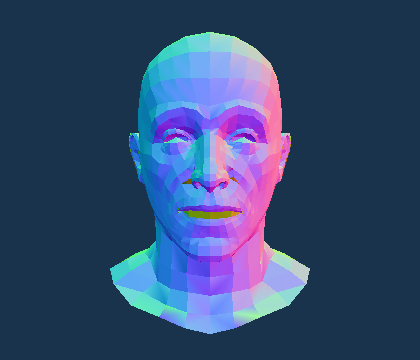
\includegraphics[width=0.35\textwidth]{./figs/o_0640.png}}
  \end{subfigure}
  
   \begin{subfigure}[]
  {\label{fig:inter3}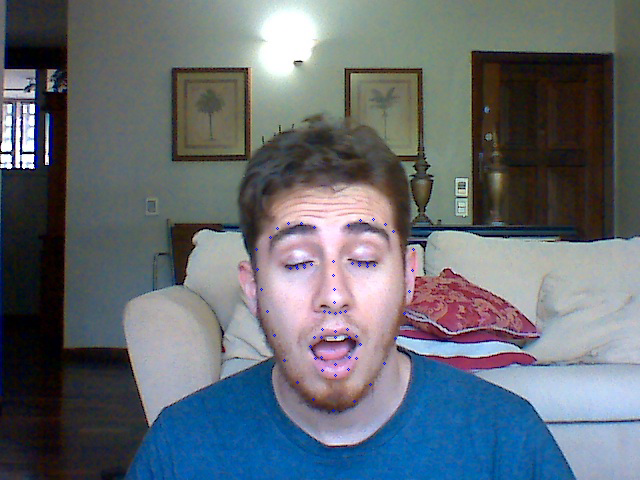
\includegraphics[width=0.35\textwidth]{./figs/i_0780.png}}
  \end{subfigure} 
  \begin{subfigure}[]
  {\label{fig:inter4}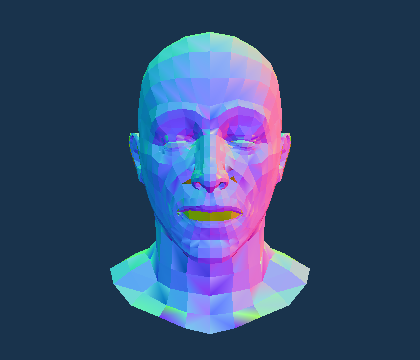
\includegraphics[width=0.35\textwidth]{./figs/o_0850.png}}
  \end{subfigure}

  \caption{Imagens que demonstram o sistema em funcionamento. Compare a Figura \ref{fig:sist-func}(d) com a \ref{fig:sist-func-2}(d) para notar que o avatar está sorrindo com a boca fechada nesta e aberta naquela. } 

  \label{fig:sist-func-2}
\end{figure}

\begin{figure}[!htb]
  \centering
  \begin{subfigure}[]{\label{fig:inter1}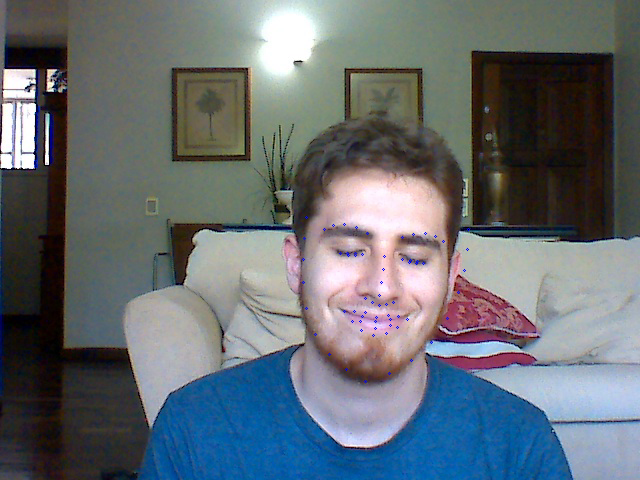
\includegraphics[width=0.35\textwidth]{./figs/i_0400.png}}
  \end{subfigure}   
  \begin{subfigure}[]{\label{fig:inter2}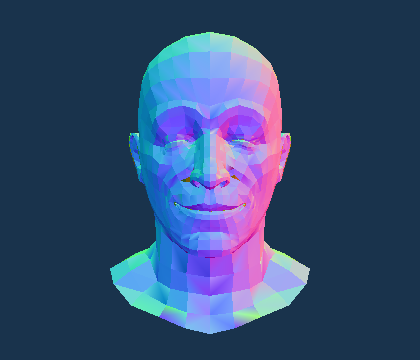
\includegraphics[width=0.35\textwidth]{./figs/o_0490.png}}
  \end{subfigure}
  
  \begin{subfigure}[]
  {\label{fig:inter3}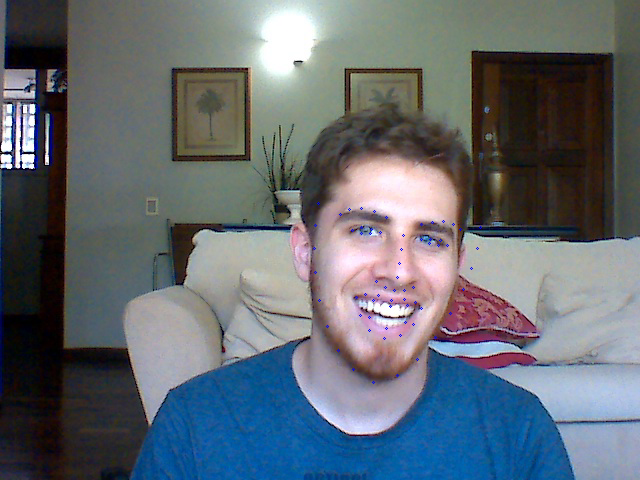
\includegraphics[width=0.35\textwidth]{./figs/i_0140.png}}
  \end{subfigure}
  \begin{subfigure}[]
  {\label{fig:inter4}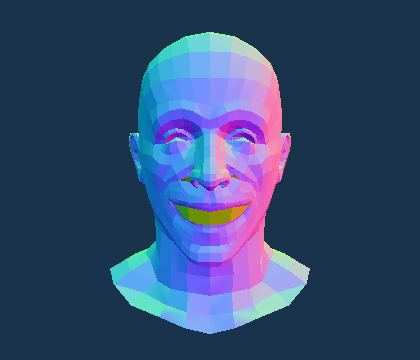
\includegraphics[width=0.35\textwidth]{./figs/o_0160.png}}
  \end{subfigure}

  \caption{Imagens que demonstram o sistema em funcionamento. Novamente, o avatar pode sorrir com a boca fechada ou com a boca aberta, podendo o olho estar fechado e aberto. As poses são combinadas independentemente.}

  \label{fig:sist-func-3}
\end{figure}

\begin{figure}[!htb]
  \centering
  \begin{subfigure}[]{\label{fig:inter1}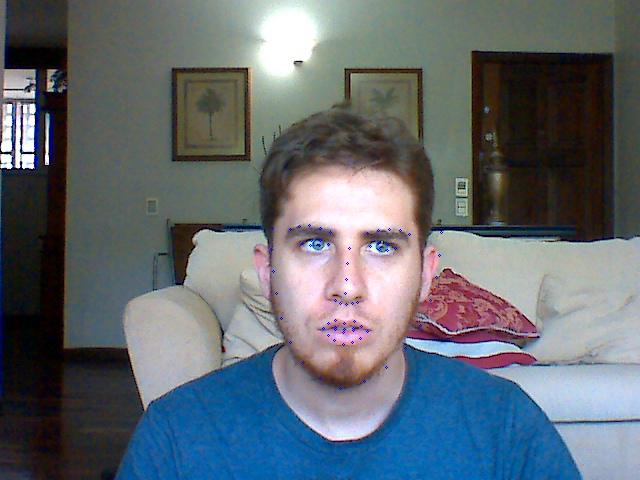
\includegraphics[width=0.35\textwidth]{./figs/i_0250.png}}
  \end{subfigure}   
  \begin{subfigure}[]{\label{fig:inter2}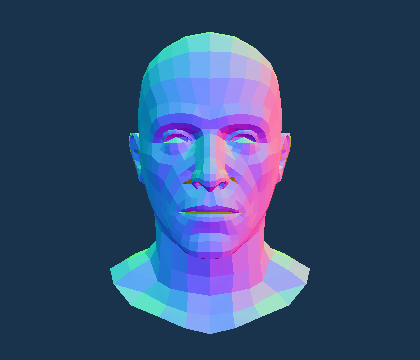
\includegraphics[width=0.35\textwidth]{./figs/o_0320.png}} 
  \end{subfigure}  
  
  \begin{subfigure}[]
  {\label{fig:inter3}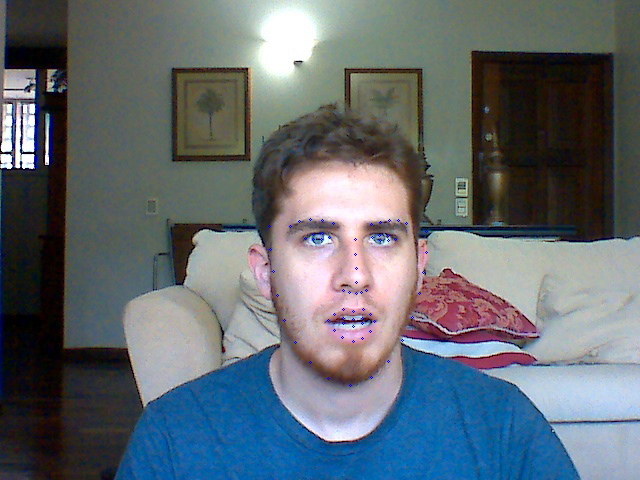
\includegraphics[width=0.35\textwidth]{./figs/i_0260.png}}
  \end{subfigure} 
  \begin{subfigure}[]
  {\label{fig:inter4}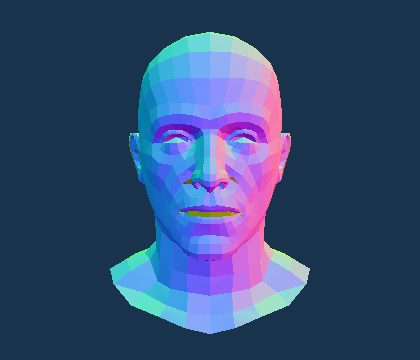
\includegraphics[width=0.35\textwidth]{./figs/o_0330.png}}
  \end{subfigure}
  
    \begin{subfigure}[]
  {\label{fig:inter4}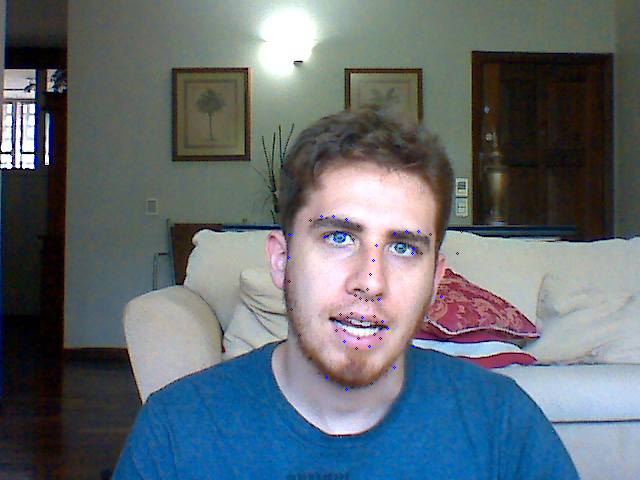
\includegraphics[width=0.35\textwidth]{./figs/i_0270.png}}
  \end{subfigure}
    \begin{subfigure}[]
  {\label{fig:inter4}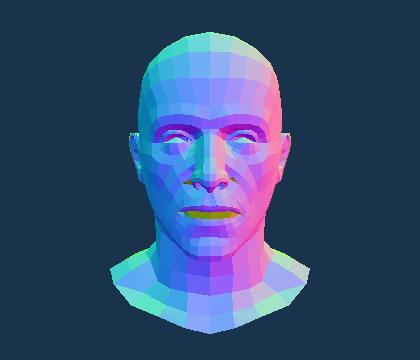
\includegraphics[width=0.35\textwidth]{./figs/o_0340.png}}
  \end{subfigure}

  \caption{Imagens que demonstram o sistema em funcionamento \textit{frame} a \textit{frame}. A sequência mostra a abertura gradual da boca enquanto o personagem conversa com as câmeras.}

  \label{fig:sist-func-4}
\end{figure}




